\documentclass[dvipdfmx]{jsarticle}

 \usepackage{ascmac}
 \usepackage{graphicx}
 \usepackage[dvipdfmx]{color}
 \usepackage{amssymb,amsmath,amsthm}
 \usepackage{graphics}
 \usepackage{fancybox, tcolorbox}
 \tcbuselibrary{raster,skins, breakable}
 \usepackage{nccmath}
 \usepackage{tikz}
 \usetikzlibrary{intersections, calc, cd}
 \usepackage{bm}
 \usepackage[italicdiff]{physics}
 \usepackage{titlesec}
 \usepackage{mathtools}
 \usepackage{enumerate}
 \usepackage{wrapfig}
 \usepackage[margin=20mm]{geometry}
 \usepackage[dvipdfmx]{hyperref}
% for hyperref
\usepackage{pxjahyper}

\title{Raman dot (Rdot) による多色細胞計測}
\author{}
\date{}
\begin{document}


\maketitle
\vspace{-60pt}
\section{モチベーション}
\begin{itemize}
  \item 従来の細胞観測は主に蛍光色素を使用.しかし,
  \begin{itemize}
    \item 染色条件や光毒性によって細胞死のリスクがある.
    \item 細胞Aと細胞Bの2群識別は容易でも,同時に10種程度の多重識別は困難.
    \item 蛍光は発光スペクトルの線幅が広く,ピークが重なってスペクトルがぼやける
  \end{itemize}
  \item ラマン散乱はピークが細いため,重なりが少なく識別しやすいピークを用いた多色化が可能.
\end{itemize}

\section{難しいこと(技術的課題)}
\begin{itemize}
  \item ラマン信号は蛍光に比べて非常に弱い(桁違いに小さい断面積).
  \item 通常は蛍光しない波長・条件でラマンを測るが,細胞イメージングでは実用上,蛍光が見える波長帯の励起を使わざるを得ない場面が多く,ラマン活用のハードルが高い.
\end{itemize}

\section{新規性(基本コンセプト)}
\begin{itemize}
  \item 色素は分子間距離が近すぎると蛍光消光(自己消光)する性質がある.
  \item そこで,色素を極高濃度に詰め込み,蛍光は意図的に抑えてラマンのみを得る戦略をとる.
  \item ただし遊離の色素は細胞毒性の懸念があるため,無機・有機ナノカプセルへ封入して生体適合性と局在制御を図る.
  \item $\Rightarrow$ 適切なカプセル材料と封入手法の探索が鍵.
\end{itemize}


\section{今回やったこと(現状)}
\begin{itemize}
  \item 既存の各種色素が所望のカプセルに自発的に入るかを実験的に調査.
  \item 結果:大半が封入されず,現行条件では実用的なロードに至らず挫折.
\end{itemize}

\section{今後すること}

\begin{wrapfigure}[10]{r}{70mm}
\centering
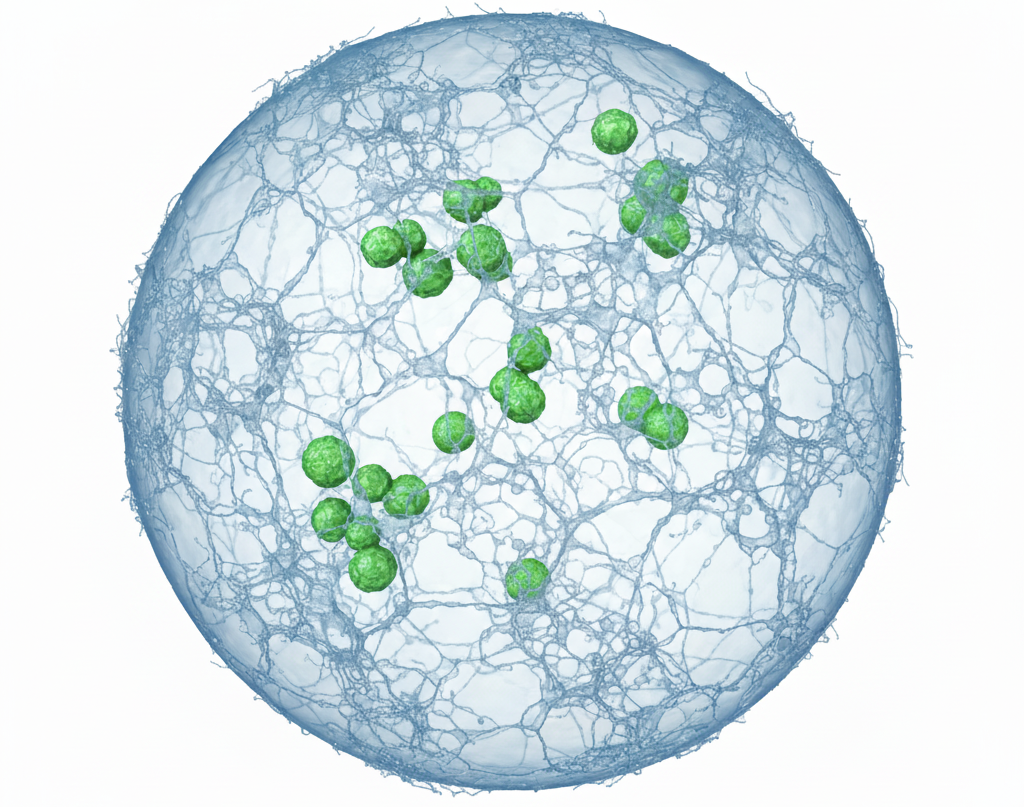
\includegraphics[scale= 0.10]{dotgraph.png} 
\caption{カプセルのイメージ}
\end{wrapfigure}

方針転換をして,
カプセルへの封入手法そのものを再設計する.
(現在水での溶媒でカプセルへの封入をしているけど,それを無極性で実行できないかを調べる)

\end{document}
